\section{Neuronales Netz}\label{sec:nn}
\subsection{Vorverarbeitung der Daten}
In der Analyse der Daten (siehe\autoref{sec:analyse}) wurde die Korrelation 
der verschiedenen Eigenschaften von Wohnungen untersucht. Die dort gefundenen
Zusammenhänge können nun verwendet werden, um die Eingaben für das Neuronale 
Netz anzupassen. Dies ist notwendig, da ein neuronales Netz effizienter
die gewünschte Funktion erlernen kann, wenn die Eingaben aussagekräftige 
Informationen darstellen. \\
Aus diesem Grund werden für das Netz nicht einfach die in der Aufgabenstellung 
gegebenen Attribute verwendet sondern Attribute die eine hohe Korrelation besitzen
zusammengefasst und Attribute die einen geringen Einfluss auf die Bewertung haben
nicht verwendet. \\
Die Folgende Auflistung zeigt die Attribute, die verwendet werden: 
\begin{itemize}\label{lst:Eigenschaften}
    \item \textbf{Kosten pro Quadratmeter:} Miete, Quadratmeter
    \item \textbf{Gesamtkosten:} Nebenkosten, Miete, Kaution
    \item \textbf{Kinderfreundlichkeit:} Schule, Kindergarten
    \item \textbf{Mobilität:} Entfernung
    \item \textbf{Ausstattung:} Möbliert
    \item \textbf{Zimmerzahl}
\end{itemize}

Ausgeschlossene Attribute mit Korrelationswerten unter 0,1 beziehungsweise -0,1 sind:\\
Stockwerk, Heizung, Hausmeister, S-Bahn, Alter, Aufzug, Lage, Küche, Bad, Balkon, Terrasse, Kehrwoche, 
und Garage.

\paragraph{Kosten pro Quadratmeter}
Dieses Attribut löst die Korrelation zwischen Miete und der Anzahl der Quadratmeter und kann 
stellt so eine aussagekräftigere Eigenschaft für die Bewertung des Preis-Leistungsverhältnisses dar.


\paragraph{Umwandlung der Daten in numerische Werte}
Im nächsten Schritt müssen alle Werte in numerische Werte umgewandelt werden. 
\begin{itemize}
    \item \textit{num-num}: Bei diesen Werten wird ganz einfach der Mittelwert gebildet. 
    \item \textit{über/unter}: Die Randwerte werden als normale Werte angesehen. 
    \item \textit{nah/erreichbar/fern}: Hier bietet es sich an das Attribut als \textit{Entfernung zu ...} umzuschreiben. 
                So kann für \textit{nah} der Minimalwert und für \textit{fern} der Maximalwert verwendet werden.
    \begin{itemize}
        \item nah: 0
        \item erreichbar: 0,5
        \item fern: 1
    \end{itemize}
    \item \textit{Boolean}: Für Werte die entweder erfüllt oder nicht erfüllt sind, wird 0 (nicht erfüllt) und 1 (erfüllt) verwendet.
\end{itemize}

Berechnungen die durchgeführt werden müssen: 
\begin{equation}
        MieteProQuadratmeter = \frac{Miete}{Quadratmeter}
\end{equation}
\begin{equation}
    Gesamtkosten = Miete + Nebenkosten + Kaution
\end{equation}
\begin{equation}
    Kinderfreundlichkeit = \frac{Schule + Kindergarten}{2}
\end{equation}

\paragraph{Normierung der Daten}
Um eine Normierung der Daten durchzuführen müssen zunächst die Maximalwerte der 
jeweiligen Attribute definiert werden. Die Werte werden anschließend auf Werte 
zwischen 0 und 1 normiert. Dies ist notwendig, da eine Vorgewichtung der Attribute
vermieden werden soll.

\subsection{Netzstruktur}
Das Netz soll aus $6$ Eingabewerten einen Ausgabewert berechnen. 
\autoref{img:nnStruktur} zeigt die Struktur des Netzes zum Lösen 
dieses Problems. 
\begin{figure}[h]
    \centering
    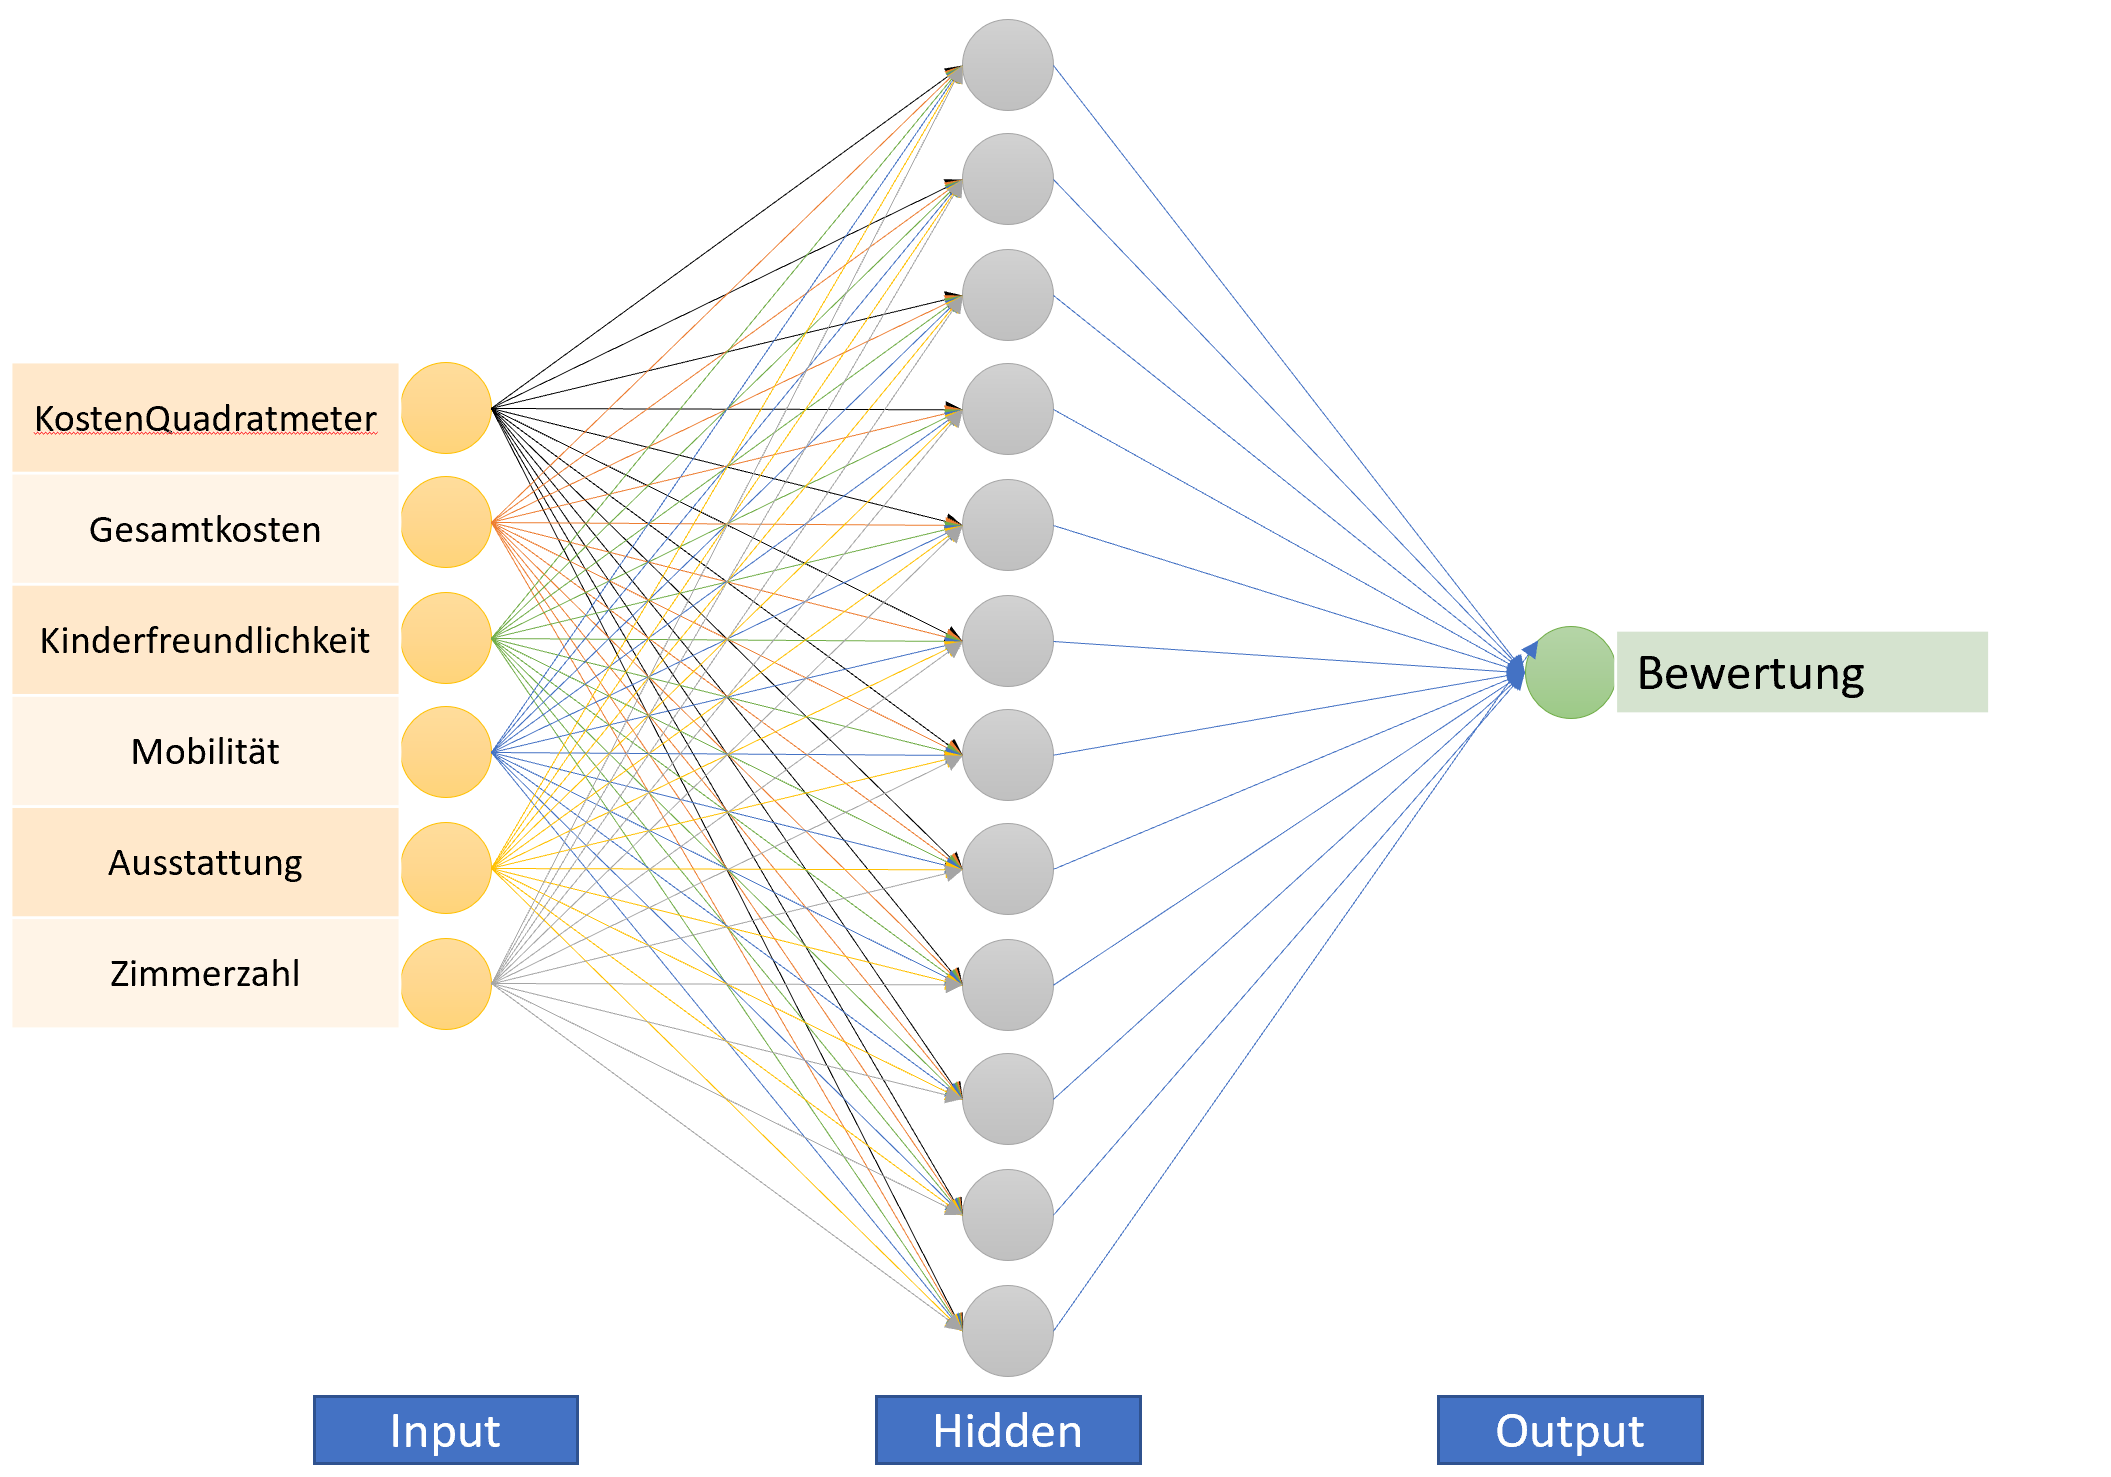
\includegraphics[width=15cm]{NNStruktur.PNG}
    \label{img:nnStruktur}
    \caption{Struktur des Neuronalen Netzes}
\end{figure}

Die \textit{Input-Layer} besitzt $6$ Neuronen, dies entspricht der 
Anzahl der Eigenschaften (siehe \autoref{lst:Eigenschaften}). 
Die Anzahl der Neuronen in der \textit{Hidden-Layer} ergibt sich aus 
$CountHidden = CountInput * 2$. Die \textit{Output-Layer} besitzt
lediglich ein Neuron, dass die Bewertung der Wohnung angibt. 

\paragraph{Initiale Gewichtung der Neuronen}
Die initialen Gewichte für das Netz werden zufällig gesetzt. Diese werden in der Lernphase 
mit hilfe einer Lernregel angepasst.

\paragraph{Aktivierungsfunktion und Schwellwert}
Die Aktivierungsfunktion eines Neurons gibt an, ab welchem Wert das Neuron das 
Signal an die nächste Schicht weiterleitet. 
Für diesen Anwendungsfall bietet sich eine Sigmoide-Funktion an, 
da diese die Eigenschaft besitzt ab dem Schwellwert allmählich 
Signale weiterzuleiten.\\

\begin{equation}
    T_s(x) = \frac{1}{1+e^(\frac{x-S}{k})}
\end{equation}

Das bedeutet, bei einem Schwellwert von $0,5$, wird ein Signal weitergeleitet. 
Allerdings erst bei einem Wert von $1$ ein maximales Signal. 
 

\paragraph{Transferfunktion}
Die Transferfunktion wandelt die normierten Eingabewerte in die Ausgabe der einzelnen Neuronen um.

\paragraph{Lernregel}
Die Lernregel sorgt für die Anpassung der Gewichte. Das hier gewählte 
Verfahren ist das \textit{Backpropagation-Verfahren}. 
Dieses Verfahren bietet sich an, da nach der Berechnung leicht der Netzfehler bestimmt werden kann. 
Der Fehler wird anschließend zurück durch das Netz propagiert und die Gewichte
werden angepasst. Die Fehlerbestimmung erfolgt schichtweiße,beginnent mit der Output-Layer, 
da hier der erwartete Wert zur Verfügung steht. Wurden die Fehler von jeder 
Schicht bestimmt, werden die Gewichte,angepasst. 
Wie die Gewichte angepasst werden zeigt \autoref{eqn:gewichte}. 
Hierbei wird das Gewicht des Neurons $j$ angepasst bei einer Eingabe, 
von Neuron $i$.
$\delta_j$ ist der Fehler des aktuellen Neurons, $x_i$ ist der Wert der von $i$ an $j$ weitergegeben wird.
$\eta_i$ ist der Lernkoeffizient. 
Dieser gibt an, wie stark die Gewichte angepasst werden und liegt zwischen 0 und 1.

\begin{equation}
    w_{ij}(t+1) = w_{ij}(t) + \eta * \delta_j*x_i
    \label{eqn:gewichte}
\end{equation}
Bei einfachen Problemen kann der Lernkoeffizent 1 sein, da das hier 
bearbeitete Problem weder besonders einfach allerdings auf der anderen Seite auch 
nicht viele Schichten notwendig sind. Bietet es sich an einen Lernkoeffizent von 
$0,7$ zu wählen. Dieser kann mit sinkendem Fehler verringert werden. 
Damit die optimale Lösung nicht übersprungen wird.

\subsection{Arbeitsweise/Ablauf}
Die folgende Auflistung zeigt, den Gesamtablauf des Netzes während eines 
Lernschrittes.
\begin{enumerate}
    \item Initialisierung
    \item Berechnung der Aktivierung \textit{Hidden-Layer}
    \item Berechnung Ausgabe der \textit{Hidden-Layer} mithilfe der Transferfunktion
    \item Berechnung Aktivierung \textit{Output-Layer}
    \item Berechnung der Ausgabe durch die Transferfunktion.
    \item Berechnung des Fehlers der \textit{Output-Layer}
    \item Berechnung des Fehlers der \textit{Hidden-Layer}
    \item Berechnung des Fehlers der \textit{Input-Layer}
    \item Anpassung der Gewichte der \textit{Output-Layer}
    \item Anpassung der Gewichte der \textit{Hidden-Layer}
    \item Anpassung der Gewichte der \textit{Input-Layer}
\end{enumerate}

\subsection{Bibliothek Tensorflow zur Implementierung}
Tensorflow ist eine Python-Bibliothek für verschiedene Anwendungen im Bereich Deep Learning. 
Der Name spiegelt das Grundkonzept dieser Bibliothek wieder. 
\textit{Tensor} bezeichnet den Datensatz der in das Deep Learning System 
eingegeben und verarbeitet wird. \textit{Flow} bezeichnet den Ablauf, 
der Verarbeitung des Datensatzes. \\
Beim Erstellen eines Systems mit Tensorflow werden zwei Phasen 
unterschieden. 
Die Bibliothek bietet neben dem generellen Konzept für Maschine Learning Anwendungen 
viele weiter mathematische Funktionen. 
\cite{tf:2018}